\section{UTILIDADES}
\subsection{Gráfico de dependencias}
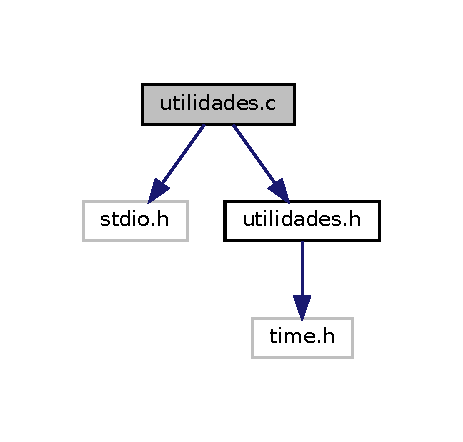
\includegraphics[width=\textwidth, angle=0, scale=0.6]{dep/utilidades_include.pdf}
\subsection{Funciones}
\begin{itemize}
    \item \cc{void flush_in(void)}
    \item \cc{void system_pause(void)}
    \item \cc{int validarFecha(char *cadena)}
    \item \cc{int validarHora(char *cadena, int hoy)}
    \item \cc{int fechaMenor(struct tm* fecha)}
    \item \cc{int fechaIgual(struct tm* fecha)}
    \item \cc{int horaMenor(struct tm* hora)}
\end{itemize}
\subsection{Definiciones}
\begin{itemize}
     \item \cc{void flush_in(void}
    \begin{itemize}
        \item \textbf{Descripción}
        \begin{itemize}
			\item Vacía el flujo de la entrada estandar.
		\end{itemize}
	\end{itemize}
    \item \cc{void system_pause(void}
   \begin{itemize}
       \item \textbf{Descripción}
       \begin{itemize}
           \item Agrega una pausa en la ejecucion.
       \end{itemize}
   \end{itemize}
   \newpage
   \item \cc{int validarFecha(char *cadena)}
    \begin{itemize}
        \item \textbf{Descripción}
        \begin{itemize}
			\item Valida una cadena con el formato dd/mm/aaaa.
		\end{itemize}
		\item \textbf{Parámetros}
		\begin{itemize}
			\item \cc{cadena} $\rightarrow$ Contiene una fecha.
		\end{itemize}
        \item \textbf{Devuelve}
		\begin{itemize}
			\item \cc{1} $\rightarrow$ Formato correcto y fecha igual a la del sistema.
            \item \cc{0} $\rightarrow$ Formato correcto.
            \item \cc{-1} $\rightarrow$ Formato incorrecto.
		\end{itemize}
	\end{itemize}
    \item \cc{int validarHora(char *cadena, int hoy)}
     \begin{itemize}
         \item \textbf{Descripción}
         \begin{itemize}
 			\item Valida una cadena con el formato hh:mm.
 		\end{itemize}
 		\item \textbf{Parámetros}
 		\begin{itemize}
 			\item \cc{cadena} $\rightarrow$ Contiene una hora.
            \item \cc{hoy} $\rightarrow$ Contiene el dia de hoy.
 		\end{itemize}
         \item \textbf{Devuelve}
 		\begin{itemize}
 			\item \cc{1} $\rightarrow$ Formato correcto.
             \item \cc{0} $\rightarrow$ Formato incorrecto.
 		\end{itemize}
 	\end{itemize}
    \item \cc{int fechaMenor(struct tm* fecha)}
     \begin{itemize}
         \item \textbf{Descripción}
         \begin{itemize}
 			\item Comprueba si la fecha es menor a la de hoy.
 		\end{itemize}
 		\item \textbf{Parámetros}
 		\begin{itemize}
 			\item \cc{fecha} $\rightarrow$ Contiene tm que contiene la fecha a comprobar.
 		\end{itemize}
         \item \textbf{Devuelve}
 		\begin{itemize}
 			\item \cc{1} $\rightarrow$ Si la fecha es menor.
             \item \cc{0} $\rightarrow$ Si la fecha es mayor o igual.
 		\end{itemize}
 	\end{itemize}
    \item \cc{int fechaIgual(struct tm* fecha)}
     \begin{itemize}
         \item \textbf{Descripción}
         \begin{itemize}
 			\item Comprueba si la fecha es igual a la de hoy.
 		\end{itemize}
 		\item \textbf{Parámetros}
 		\begin{itemize}
 			\item \cc{fecha} $\rightarrow$ Contiene tm que contiene la fecha a comprobar.
 		\end{itemize}
         \item \textbf{Devuelve}
 		\begin{itemize}
 			\item \cc{1} $\rightarrow$ Si la fecha es igual.
             \item \cc{0} $\rightarrow$ Si la fecha es mayor o menor.
 		\end{itemize}
 	\end{itemize}
    \item \cc{int horaMenor(struct tm* hora)}
     \begin{itemize}
         \item \textbf{Descripción}
         \begin{itemize}
 			\item Comprueba si una hora es menor a la hora actual del sistema.
 		\end{itemize}
 		\item \textbf{Parámetros}
 		\begin{itemize}
 			\item \cc{hora} $\rightarrow$ Contiene tm que contiene la hora a comprobar.
 		\end{itemize}
         \item \textbf{Devuelve}
 		\begin{itemize}
 			\item \cc{1} $\rightarrow$ Si la hora es menor.
             \item \cc{0} $\rightarrow$ Si la hora es mayor o igual.
 		\end{itemize}
 	\end{itemize}
\end{itemize}
\newpage
